\documentclass[a4paper,draft]{article}

\usepackage[utf8]{inputenc}
\usepackage[T1]{fontenc}

\usepackage{roboto}
\usepackage{mathptmx}
\usepackage{tgtermes}
\usepackage{amsmath}
\usepackage{amssymb}
\usepackage{stmaryrd}

\usepackage{mathtools}
\usepackage{amsthm}
\usepackage{thmtools}
\declaretheorem{theorem}
\declaretheorem{lemma}
\declaretheorem{corollary}
\declaretheorem[style=definition,qed=$\blacktriangle$]{example}
\declaretheorem[style=definition,qed=$\blacktriangle$]{definition}
\numberwithin{equation}{section}

\usepackage{enumitem}
\setlist[enumerate,1]{label=\alph*)}
\newlist{prfcases}{enumerate}{1}
\setlist[prfcases,1]{label={\it Case \arabic*.},align=left,leftmargin=\parindent,itemindent=*}

\newenvironment{isabelle}{\list{}{}\item\relax}{\endlist}
\newcommand{\iindent}{\-\hspace{1em}}

\usepackage{algorithm}
\usepackage[final]{listings}
\lstset{numbers=left,firstnumber=1,stepnumber=5,numberfirstline,
	basicstyle=\ttfamily\small,keywordstyle=\ttfamily\small\itshape,columns=flexible}

\usepackage{tikz}
\usetikzlibrary{shapes.geometric,matrix,decorations.pathreplacing}
\tikzset{itermtree/.style={level distance=6mm,sibling distance=10mm,%
	edge from parent/.style={draw,solid},every node/.style={solid}}}
\tikzset{pure/.style={draw,rectangle,inner sep=4pt,minimum size=5mm}}
\tikzset{term/.style={draw,circle,inner sep=1pt,minimum size=5mm}}
\tikzset{ap/.style={fill,diamond,inner sep=0pt,minimum size=6pt}}
\tikzset{subtrm/.style={draw,isosceles triangle,isosceles triangle apex angle=55,%
	shape border rotate=90,minimum height=10mm,anchor=north,child anchor=north}}
\tikzset{subtrmf/.style={subtrm,level distance=10mm,sibling distance=16.67mm}}
\tikzset{subtrmn/.style={subtrm,level distance=4mm,sibling distance=6.67mm}}
\tikzset{abbrv/.style={dashed}}

\usepackage[english]{babel}
\hyphenation{Isa-belle}

\usepackage[
	style=numeric,
%	sorting=none,
	doi=false,
	urldate=long,
]{biblatex}
\addbibresource{bibliography.bib}

\usepackage[hidelinks]{hyperref}


\newcommand{\ldb}{\llbracket}
\newcommand{\rdb}{\rrbracket}
\newcommand{\todo}{\fbox{To do.}}

\newcommand{\oftype}{\mathrel{::}}
\newcommand{\funT}{\Rightarrow}
\newcommand{\abs}[2]{\lambda #1.\>#2}
\newcommand{\Imp}{\Longrightarrow}
\newcommand{\imp}{\longrightarrow}
\newcommand{\Iff}{\Longleftrightarrow}
\newcommand{\All}[2]{\bigwedge #1.\>#2}
\newcommand{\all}[2]{\forall #1.\>#2}
\newcommand{\tvar}[1]{{'\!\textit{#1}}}
\newcommand{\svar}[1]{\textit{?#1}}
\newcommand{\set}[2]{\{#1\mid #2\}}

\DeclareMathOperator{\pure}{\mathit{pure}}
\newcommand{\ap}{\diamond}
\DeclareMathOperator{\sterm}{\mathsf{term}}
\DeclareMathOperator{\spure}{\mathsf{pure}}
\DeclareMathOperator{\sivar}{\mathsf{var}}
\newcommand{\siabs}[2]{\mathsf{abs}\;#1.\>#2}
\newcommand{\sap}{\mathbin{\mathsf{`ap`}}}
\newcommand{\sapp}{\>}
\newcommand{\sabs}[2]{{\boldsymbol\lambda} #1.\>#2}
\newcommand{\tabs}[2]{{\boldsymbol\lambda}^\ast #1.\>#2}
\newcommand{\termeq}{=_{\alpha\beta\eta}}
\newcommand{\unlift}[1]{\left\downarrow #1\right.}
\DeclareMathOperator{\vars}{var}
\newcommand{\varseq}{\overrightarrow{\vars}}
\DeclareMathOperator{\abseq}{abs}


\title{Applicative Functors in Isabelle/HOL}
\author{Joshua Schneider}

\begin{document}

\begin{titlepage}\sf\large\raggedleft
\makeatletter
{\huge\bfseries\@title} \\
\vspace{7mm}
{\Large\@author} \\
\vspace{2cm}
Bachelor Thesis \\
(11-947-173) \\
\vspace{7mm}
\@date
\makeatother

\vspace{\fill}
Advisors: \\
Prof.\ Dr.\ David Basin \\
Dr.\ Andreas Lochbihler \\
\vspace{1cm}
Department of Computer Science, ETH Zürich
\end{titlepage}

\section*{Abstract}

Applicative functors can be found in different contexts.
In functional programming, they abstract the addition of effects to types.
But also rather mathematical constructs like sets and infinite containers
are examples.
The key property of applicative functors is that they lift functions
to effectful computations.

We present a proof method based on applicative lifting, implemented for the
Isabelle/HOL proof assistant.
Hinze showed that properties of functions are often preserved when lifted.
While functors are represented naturally in the types of HOL, it is not
directly possible to reason based on this insight.
We propose an algorithm which computes a certain normal form of applicative
expressions, together with a checked proof of equivalence.
We explain formally how this normal form solves lifted equations.
For further flexibility, we take some ideas from combinatory logic:
Variables can be eliminated from applicative expressions by means of abstraction
algorithms.
This second approach takes the nuances of the particular functors into
consideration.
Together, we provide the development as a ready-to-use package for Isabelle.
We demonstrate it on algebraic structures lifted to streams and cotrees.


\pagebreak
\tableofcontents
\pagebreak
\section{Introduction}\label{sec:introduction}

\subsection{Motivation}\label{subsec:motivation} % TODO change?

Interactive theorem provers emphasize the human aspect of mathematical work.
Rather than relying on fully automatic proof search, the user guides
the process with their own understanding~\cite{harrison07}.
This requires a sufficiently expressive interface with features beyond plain
logical calculus.
In particular, there exists a demand for automation and abstraction of
patterns~\cite{bourke12}.
It is thus common to extend proving environments with (sometimes
domain-specific) tools.

In this report we present a particular variant of lifting we have implemented
for the Isabelle/HOL proof assistant~\cite{npw02}.
The term ``lifting'' is used in different contexts, often informally.
It vaguely refers to the transfer of mathematical objects between domains,
while preserving a certain relationship.
A concrete example are lifts of paths in topology. % TODO cite
There is also an existing Isabelle package~\cite{huffman13}, which lifts
definitions to quotient types.
Here we consider a slightly different meaning of lifting:
The transfer of operations and their properties to generic structures.
Since HOL is a typed logic, it is natural to represent these structures as
parametric types.
Let us look at a simple example.

\begin{example}\label{exmp:set-intro}
For each type $\alpha$ there is a corresponding type $\alpha\,\mathit{set}$
of sets with elements from $\alpha$.
Addition $(+)$ is a binary operator defined on natural numbers, amongst others.
How could addition of sets of natural numbers be defined, such that some
relation to $+$ remains?
The canonical way to combine two sets into a set of pairs is the cartesian
product.
Therefore, we define
\begin{equation}\label{eq:set-plus-exp}
	X \oplus Y = \set{x + y}{x \in X,\, y \in Y}.
\end{equation}
We interpret $\oplus$ as the lifting of $+$ to sets.
Note that similar definitions are possible for other operators like
multiplication, and also other element types such as real numbers.
A property of addition is associativity,
\begin{equation}\label{eq:plus-assoc}
	\all{x y z}{(x + y) + z = x + (y + z)}.
\end{equation}
It can be translated to sets of natural numbers,
\begin{equation}\label{eq:set-plus-assoc}
	\all{X Y Z}{(X \oplus Y) \oplus Z = X \oplus (Y \oplus Z)},
\end{equation}
where it holds as well, as one can check with a slightly laborious proof.
The two sides of the latter equation can be regarded as functions with three
arguments.
They are the lifted counterparts of the former equation.
\end{example}

Hinze~\cite{hinze10} came across similar patterns and proceeded to investigate
the conditions under which lifted equations are preserved.
He noticed that lifting can be defined in an intuitive fashion if the target
structure is an applicative functor~\cite{mcbride08}.
These come with two constants, usually denoted $\pure$ and $\ap$ (``ap''),
which lift a single object and the notion of function application, respectively.
Applicative functors must also satisfy some properties, which we restate in
Section~\ref{subsec:applicative}.

Every monad is an applicative functor.
Monads are a common mechanism for handling effects in functional
programming~\cite{wadler95}.
Such being the case, they are also useful for modelling in the context of
verification.
The difference between monads and applicative functors is that the latter
do not allow sub-computations to depend on previous results.
From there we can borrow quite a few examples of applicative functors:
Sum types with one variable type (known as \textsf{Either} in Haskell),
the reader monad or environment functor, the exception/backtracking list
monad~\cite{wadler85}, the state monad, and parser combinators.
Hinze originally worked on streams (infinite lists) and infinite
trees~\cite{hinze08,hinze09}.
We conclude that there are indeed relevant applicative functors, which supports
the argument that this kind of lifting is a useful abstraction.

\addtocounter{example}{-1}
\begin{example}[continued]
Back to sets, we obtain an applicative functor if $\pure$ is the singleton set
constructor $x \mapsto \{x\}$;
$F \ap X$ takes a set of functions $F$ and a set of arguments $X$
with compatible type, applying each function to each argument:
\begin{equation}\label{eq:set-ap}
	F \ap X = \set{f x}{f \in F,\, x \in X}.
\end{equation}
Now we can express lifted addition directly in terms of the base operation:%
\footnote{As customary in HOL, we treat binary operators as curried functions.}
\begin{equation}\label{eq:set-plus}
	X \oplus Y = \pure{(+)} \ap X \ap Y.
\end{equation}
(The operator $\ap$ is left-associative.)
This definition is equivalent to the previous one \eqref{eq:set-plus-exp},
but not specific to sets anymore.
\end{example}

As we have seen earlier, lifting can be generalized to equations.
One of Hinze's results is that a fundamental relationship exists between the
associative properties \eqref{eq:plus-assoc} and~\eqref{eq:set-plus-assoc}%
---the lifted form can be proven for all applicative functors, not just
$\mathit{set}$.
Moreover, this is possible for other equations as well, but not all equations
can be lifted in all functors.
Stronger conditions are required if the list of quantified variables is
different for each side of the equation.
(The left-to-right order is relevant, but not the nesting within the terms.)
These conditions must basically ensure that the functor does not add ``too many
effects'' which go beyond the simple embedding of a base type.
Such effects may be evoked if a variable takes an impure value, i.e., a value
which is not equal to $\pure x$ for any $x$.
Hinze showed that sufficient conditions can be expressed in terms of combinators
as known from combinatory logic.

These findings justify direct proofs of lifted equations.
It desirable to enable such reasoning in a proof assistant.

\begin{example}\label{exmp:set-counterexmp}
We try to lift the fact that zero is a left absorbing element for
multiplication of natural numbers, $\all{x \oftype \mathit{nat}}{0 \cdot x = 0}$,
to sets.
Note that the variable $x$ occurs only on the left.
But the lifted equation does not hold: If $x$, now generalized to
$\mathit{nat}\,\mathit{set}$, is instantiated with the empty set, then
\[ \pure{(\cdot)} \ap \pure 0 \ap \{\} = \{\} \ne \pure 0. \]
Here the effect of $\{\}$ is that it cancels out everything else if it occurs
somewhere in an lifted expression.
This makes it impossible to lift any equation with a variable occuring only on
one side to $\mathit{set}$.
We will see that other functors permit this lifting.
\end{example}


\subsection{Contributions and Overview}\label{subsec:contrib-overview}

Our primary goal is to provide an Isabelle/HOL proof method which reduces
lifted equations to their base form.
The method can be instantiated for arbitrary applicative functors.
Then the user is able to prove the lifted equations directly without having to
invent a specific proof strategy, or even simulate the approach taken here.
Apart from the theoretical appeal of the method, the resulting proof text is
usually more concise, due to the higher level of abstraction.
Together with some infrastructure, the proof method forms a basic package
for reasoning with applicative functors.

Hinze's work is the basis for the package.
He has identified the suitability of applicative functors and shown
necessary conditions for lifting of equations.
However, we needed to adapt the details to the HOL environment in order to
construct actual proofs.
This construction is directly programmed on top of Isabelle's ML interface.
We have therefore derived the correctness and some other properties of our
approach formally using a simplified calculus.
Moreover, we have further extended the idea of combinators as building blocks
for lifting, generalizing Hinze's model conditions.
Consequently, the package supports several combinator sets which functors may
exhibit, each capable of lifting different sets of equations.
A particular motivation for our package are arithmetic operations on streams
and infinite trees.
We have proven some of their properties as a usage example.

The remainder of this report is organized as follows:
The present section concludes with some background information on Isabelle/HOL,
applicative functors, and a concrete definition of lifting.
Section~\ref{sec:design} describes the design considerations, discusses the
choice of embedding, and provides a high-level overview of the proof method.
In the next two sections, we present the details of the two strategies we
have implemented:
Section~\ref{sec:normal-form} shows an implementation of the normal form of
lifted expressions;
Section~\ref{sec:combinators} is concerned with combinators and the application
of bracket abstraction to applicative terms.
\todo\ application example, related work, conclusion


\subsection{Proving with Isabelle/HOL}\label{subsec:isabelle}

Isabelle was originally designed as a framework for interactive theorem
proving, without being restricted to a specific logical system~\cite{paulson90}.
However, one chooses a particular object-logic in order to construct a theory
and prove theorems.
In this paper, we focus on the Isabelle/HOL object-logic~\cite{npw02}.
It implements the higher-order logic which was used in the HOL~system,
another proving environment~\cite{gordon93}.
Isabelle/HOL (or HOL from here~on) is arguably the most popular object-logic
of Isabelle, as it comes with an extensive library of readily formalized
mathematics.
It also supports modelling of functional programs by means of datatypes and
recursive functions, making it suitable for verification tasks. % TODO cite?

The basis of HOL is a slightly extended variant of simply-typed lambda calculus.
Therefore, every object (and every term representing such an object) has a
certain type attached to it.
We use lower-case greek letters $\alpha$, $\beta$, $\gamma$ as meta-variables
for types.
The language of types consists of base types, type variables, and compound
types.
Base types are represented by their name and include fundamental types like
the booleans $\mathit{bool}$ and the natural numbers $\mathit{nat}$.
Type variables stand for an arbitrary types.
In Isabelle syntax, they are distinguished by a prefixed `$'$', e.g.
$\tvar{a}$, $\tvar{b}$, $\tvar{c}$.
The polymorphism in HOL is quite restricted, though, because higher-ranked
types cannot be expressed:
There is no explicit quantifier on the type level.
This rules out functions which take a polymorphic function as an argument and
apply it to values of different types.
Compound types are built up of a type constructor and a list of types.
The type constructor determines the number of argument types.
For example, the unary type constructor $\mathit{set}$ denotes sets with
elements of a certain type.
The argument is written on the left as in $\mathit{nat\,set}$, the type of
sets of natural numbers.
Multiple types are written in parentheses: $(\alpha, \beta) \mathit{fun}$.
$\mathit{fun}$ is the special type constructor for (total) functions from
$\alpha$ to $\beta$.
More commonly, the infix operator $\funT$ is used.
It is right-associative, i.e. $\alpha \funT \beta \funT \gamma$ is notation for
$(\alpha, (\beta, \gamma) \mathit{fun}) \mathit{fun}$.
Note that type constructors are different from types and must always be
concrete.
In particular, it is not possible to use a variable in place of a type
constructor!

Terms follow the standard rules of lambda calculus.
Atomic terms are constants and variables.
Application of a function $f$ to an argument $x$ is written $f\,x$.
Functions with multiple arguments are commonly curried in HOL;
we can drop parentheses accordingly: $f\,x\,y$ is the same as $(f\,x)\,y$.
Abstraction of a term $t$ over the variable $x$ is written $\abs{x}{t}$.
Terms must be well-typed, of course.
The types of variables and polymorphic constants can usually be omitted, since
they are inferred automatically.
Explicit type constraints are denoted by $t \oftype \alpha$ and may occur
anywhere in a term.
While all terms are represented internally roughly as shown above, Isabelle
comes with extensible notation support.

\begin{example}\label{exmp:hol-terms}
We already introduced the type $\mathit{nat}$.
Number literals can be used directly.
Common arithmetic operators are available, like%
\footnote{These functions actually have a more generic type (they are
overloaded). We will look at this later on.}
$\mathit{plus} \oftype \mathit{nat} \funT \mathit{nat} \funT \mathit{nat}$.
We can also use infix operators:
\[ \abs{(x \oftype \mathit{nat})\,y}{1 + x * y} \]
is a function which multiplies two natural numbers and adds one to the result.
Another important type family are sets.
They can be specified as finite collections $\{\}$, $\{a, b, c\}$ etc., and
by using set comprehension:
Let $P$ be a predicate $\alpha \funT \mathit{bool}$.
Then $\{x.\; P x\}$ is the set of those values $x \oftype \alpha$ such that
$P x$ is true, and $\set{f x}{x.\; P x}$ is the image of that set under $f$.

Logical formulas are centered around truth values.
Thus, the usual connectives like conjunction $\land$ and implication $\imp$
operate on type $\mathit{bool}$.
Quantifiers work just as expected: The term
\[ \all{(x \oftype \mathit{nat})\,y}{x + y = y + x} \]
states that addition of natural numbers is commutative.
Note that $=$ is just another operator of polymorphic type
$\tvar{a} \funT \tvar{a} \funT \mathit{bool}$.
Internally, quantifiers are represented as constants applied to lambda
abstractions, which handle the variable binding.
\end{example}

In order to support different object-logics, Isabelle contains an immediate
layer, the meta-logic Pure (see e.g. \cite[Chapter~2]{implementation-ref}).
It is an ``intuitionistic fragment of higher-order logic''~\cite[27]{isar-ref}.
Pure has two main uses within the Isabelle framework: representation and
manipulation of deduction rules, and goal states.
While our user interface is intended to be used with HOL, the underlying
theorems are always represented as propositions of Pure.
Therefore it plays an ancillary role in our tool.
The following operators are separate from those of HOL:
meta-quantification $\bigwedge$ instead of the universal quantifier $\forall$,
and meta-equality $\equiv$ instead of $=$.
Each of these are logically equivalent, though.
In particular, the generic rewriting and simplification tools work with $\equiv$.
As an example of Pure, consider the symmetry axiom for $\equiv$ in traditional
rule format,
\[ \frac{\Gamma \vdash x \equiv y}{\Gamma \vdash y \equiv x}. \]
Deduction in Isabelle handles the context $\Gamma$ automatically, and
therefore does not have to be stated in the corresponding proposition.
The dependency of the conclusion on the hypothesis translates to
meta-implication;
the outermost meta-quantified variables (and all type variables) % FIXME
are turned into schematic variables, which are free variables distinguished by
the prefix $\svar{}$.
Thus, the symmetry axiom appears as the theorem
\[ \mathtt{symmetric}:\quad \svar{x} \equiv \svar{y} \Imp \svar{y} \equiv \svar{x}. \]
Schematic (type) variables are eligible for instantiation by some core
functions. % FIXME

Isabelle is an LCF-style prover, i.e., proofs are composed by invoking
trusted, primitive inferences programmed in the implementation language
SML, at least on the lowest level.
For instance, the symmetry axiom is available in combination with modus ponens
as the function \verb|Thm.symmetric|, which takes a theorem $x \equiv y$ and
returns a new theorem $y \equiv x$.
The function is part of the large SML interface of Isabelle, which not only
constitutes its implementation, but can also be used for new tools.

In contemporary use of Isabelle, user input to the system is expressed in
the Isar language~\cite{wenzel99,wenzel02,isar-ref}.
It aims to encode proofs in a way that is formal, i.e. has precise semantics,
but still resembles informal patterns of reasoning.
The basic organization unit in Isar is a theory.
The body of a theory consists of a sequence of commands, which consecutively
augment the logical context by declarations of various kinds.
Other theories may be imported in the beginning, leading to a acyclic graph
of theory dependencies.
The set of data stored within a theory can be extended through the programming
interface.
This is relevant to us, because it allows us to register applicative
functors in the theory context.

Commands constitute the so-called outer syntax of Isar.
Terms and types occuring within them are parsed separately, according to the
inner syntax.
In certain cases, a command may put the theory state into proof mode.
After the proof is finished, the associated goal becomes a fact, which can be
further handled by some associated code.
The important \textbf{lemma} family of commands works this way, for example.
New commands are frequently introduced for specifications.
For example, algebraic datatypes can be defined with the \textbf{datatype} command.
Finally, there are other extensible syntactical categories which are commonly
used in Isar:
Proof methods denote (possibly parameterized) operations on the goal state
within a regular Isar proof.
These operations are provided by arbitrary code and thus can be arbitrarily
complex.
Attributes invoke further processing steps on already proven facts, either
transforming them or causing additional declarations to the context.


\subsection{Applicative Functors and Lifting}\label{subsec:applicative}

Applicative functors were introduced by McBride and Paterson~\cite{mcbride08}
in order to abstract a recurring theme they observed in the programming language
Haskell.
In fact, their findings already included some examples of lifting.
They defined an applicative functor as a unary type constructor $f$ with
associated constants
\begin{align*}
	\pure_f &\oftype \alpha \funT \alpha f, \\
	(\ap_f) &\oftype (\alpha \funT \beta) f \funT \alpha f \funT \beta f.
\end{align*}
We omit the subscripts if the functor is clear from the context.
Moreover, the following laws must be satisfied:
\begin{align*}
	\tag{identity} \pure{\mathit{id}} \ap u &= u \\
	\tag{composition} \pure{(\cdot)} \ap u \ap v \ap w &= u \ap (v \ap w) \\
	\tag{homomorphism} \pure{f} \ap \pure x &= \pure{(f x)} \\
	\tag{interchange} u \ap \pure{x} &= \pure{(\abs{f}{f x})} \ap u
\end{align*}
We have already seen how the two constants can be used to build terms.
McBride and Paterson coined the term ``idiom'' to refer to a particular
interpretation of such terms.
In line with Hinze, we will use ``applicative functor'' and ``idiom''
interchangeably.

The identity type constructor defined by $\alpha\,\mathit{id} = \alpha$ is a
trivial applicative functor for $\pure{x} = x$, $f \ap x = f x$.
We can take any abstraction-free term $t$ and replace each constant $c$ by
$\pure{c}$, and each instance of function application $f x$ by $f \ap x$.
The rewritten term is equivalent to $t$ when interpreted in the identity idiom.
By choosing a different idiom, we obtain a different interpretation of the same
term structure.
In fact, this is exactly how we define the lifting of $t$.
However, the terms we are interested in can also contain variables:
Equations such as~\eqref{eq:plus-assoc} are universally quantified.
For the purpose of lifting, we ignore quantifiers and treat their variables
as free.
Like in Example~\ref{exmp:set-intro}, the variables of lifted equation should
range over the lifted type.
Note that these can take impure values.
A term consisting only of $\pure$ and $\ap$ applications and free variables is
then called an \emph{idiomatic expression}.

Every idiom is a functor, of course, and thus can be mapped over.
One obtains an equivalent formalization of idioms:
\begin{alignat*}{2}
	\mathit{map}_f &\oftype (\alpha \funT \beta) \funT \alpha f \funT \beta f, &\qquad
		\operatorname{\mathit{map}}_f\,g\,x &= \pure g \ap x, \\
	\mathit{unit}_f &\oftype () f, &\qquad \mathit{unit}_f &= \pure{()}, \\
	(\star_f) &\oftype \alpha f \funT \beta f \funT (\alpha, \beta) f, &\qquad
		x \star_f y &= \pure{(\abs{x y}{(x,y)})} \ap x \ap y.
\end{alignat*}
Some of Hinze's proofs make use of these definitions.
Dealing with product types can be a bit cumbersome in HOL, though.
The curried interface therefore seems to be a better choice, and we will
focus solely on that.

\chapter{Requirements and Basic Design}\label{sec:design}

\section{Requirements}\label{subsec:requirements}

The following is the minimal set of user actions our Isabelle package shall
support:

\begin{enumerate}
\item Declare applicative functors to the theory context.
	Given a type constructor $f$, the functions $\pure_f$ and $\ap_f$, and
	proofs for the relevant functor laws, the functor is registered with the
	package such that it can be used in subsequent invocations of the
	proof method.
\item Prove lifted equations $a'[\vec{x}] = b'[\vec{x}]$, where $a'$ and $b'$
	are idiomatic expressions with free variables $\vec{x}$, using the base
	equation $\all{\vec{y}}{a[\vec{y}] = b[\vec{y}]}$.
	More precisely, if there is a subgoal stating the former, applying the
	proof methods transforms the goal state to the latter.
	The functor should either be detected automatically, or be specified
	by the user.
\end{enumerate}

The first requirement ensures that our package is reusable, while the second
is the core functionality.
However, usability is also a concern: In the realm of interactive theorem
proving, it is not sufficient to just verify formal objects---we are not
extending the logic, after all, but providing a shortcut following a certain
principle.
We must balance the clarity of the resulting proof document and the amount of
work that the user has to put into developing a proof.
The following features are possible extensions which may help in this regard:

\begin{enumerate}
\setcounter{enumi}{2}
\item\label{itm:feat-const}
	Declare lifted constants and other terms to the theory context.
	Generally speaking, if a term $t$ with free variables $v_i$ can be expressed
	as $\pure t' \ap v_1 \ap \cdots \ap v_n$ for some $t'$, then the
	corresponding equation can be registered.
	The proof methods rewrite with these equations at the beginning,
	such that the base equation will refer to $t'$.
	This way, the user does not have to transform everything into idiomatic
	format first.
\item\label{itm:feat-flex}
	More flexibility regarding the logical structure of the input proposition.
	This includes bound variables (quantified by $\forall$ or $\bigwedge$),
	complex subgoals with premises, and cases where the variables of the lifted
	equation have been substituted by some terms.
\item\label{itm:feat-tools}
	Related proof methods and attributes, for example for forward lifting
	of facts stating a base equation.
\item\label{itm:feat-debug}
	Inspection and tracing output.
	This is particular useful if something does not work as expected.
\item\label{itm:feat-xprops}
	Extend the notion of lifting beyond equations.
	It is possible to define lifting for other logical operators.
	For example, the cancellation law $a + b = a + c \longrightarrow b = c$
	consists of two equations, joined by implication.
	We can interpret it in different domains, e.g., for integers and for
	streams of integers with element-wise addition.
	In this example, the law is true for both interpretations.
	We are not able to handle such propositions with a method just for
	equations.
\end{enumerate}

The current version at the time writing supports \ref{itm:feat-const} and
\ref{itm:feat-flex}, as well as the forward lifting described in~\ref{itm:feat-tools}.
In the remainder of this section, we will explain the design decisions we
have made in order to fulfill the requirements.
Furthermore, the registration infrastructure and the basic proof approach are
explained.


\section{Choice of Embedding}\label{subsec:embedding}

The basic principle of proof composition in Isabelle is resolution with a proven
theorem, using it as a rule of inference.
Here we argue that it is not possible to prove lifting as a single theorem, and
then we discuss potential remedies.
We are interested in applicative functors on the type level, where application
is based on the standard function space.
Therefore, each idiom comes with a type family which is indexed by a
distinguished type variable, and the related functions and laws are polymorphic
in this index.
This is the natural form of idioms in the HOL libraries; all examples mentioned
in Section~\ref{subsec:motivation} are parametric datatypes.
The proof method should work directly with equations involving these.
Regardless of the mechanism of proof construction, it needs a type constructor
as a parameter.
This concept is foreign to the type system of Pure and HOL---%
we already referred to the fact that type constructors are fixed.
Another issue is the lack of polymorphism in the inner logic:
We cannot have, say, a schematic variable \textit{?pure} and use it with
different types within the same proposition or proof.

One solution is to define a custom logic, including a term language, axioms
and meta theorems, and formalize it using the available specification tools.
In our case, the language is that of idiomatic expressions,%
\footnote{Base equations can be interpreted as expressions in the identity idiom.}
the axioms describe an equality judgment which is compatible with the
applicative functor laws, and lifting of equations is a theorem.
This is a \emph{deep embedding} of the logic~\cite{wildmoser04}.
With its tools for algebraic datatypes and recursive functions, reasoning about
such an embedding is quite manageable in HOL.
However, we want to prove propositions involving objects of HOL itself, not just
their encodings in the embedded language.
Some machinery, known as reflection, needs to perform the encoding and transfer
back results.
It must be implemented necessarily outside of the logic, but can be generic.
Chaieb and Nipkow have implemented a proof procedure using a deep embedding and
reflection in Isabelle~\cite{chaieb05}.
They point out that their approach also functions as a verification of the
proof procedure, is portable and has smaller proofs than those obtained by
automating inference rules.
Their reflection system does not support polymorphism to the extent we need,
though.

The package for nonfree datatypes~\cite{schropp13} is deeply embedded as well.
Its constructions must work with arbitrary types.
In the underlying framework, Schropp~\cite{schropp12} proposed the use of a
``pseudo-universe'', a sum type combining all relevant types.
The meta-theory of the package carries a type parameter which is instantiated
with a suitable pseudo-universe for every construction.
It may be possible to use the same approach for idiomatic expressions, since the
number of types occuring in an idiomatic expression is finite.
This number can be linear in the size of the expression, though, which bloats
the intermediate terms during reflection.
A bigger problem is the axiomatization of idioms.
For instance, the identity law would refer to a function of type $\alpha \funT \alpha$
for each type $\alpha$ in the pseudo-universe.
Thus, the universe needs to be closed under function types.
It is not clear to the author how this could be modelled.

A different approach, which is the one we will take, is a \emph{shallow embedding}.
The formulas (here, idiomatic terms) are expressed directly in the language of HOL.
Due to aforementioned restrictions, meta-theorectical results must be provided
in specialized form for each case.
We use the powerful ML interface of Isabelle to program the proof construction,
composing inferences according to the structure of the input equation.
The handling of polymorphism is simplified, as we have full control over
term and theorem instantiations.
The system still verifies the soundness of the synthesized proofs.
On the other hand, one has to assert externally that the construction algorithm
itself is correct, i.e., complete.
The main part of this report therefore justifies these algorithms.


\section{Proof Strategy}\label{subsec:proof-strategy}

The ML code of the package can be considered in two parts.
One is concerned with registration of idioms and access to the recorded
information, the other provides the actual proof methods.
We start with a summary of the former component.
It does not only store the idioms declared with the \textbf{applicative}
command (see Section~\ref{subsec:user-interface}), but also deals with the high
degree of polymorphism.
First, we need to represent the concept of an idiom.
Instead of a plain type constructor we use type schemes $f[\tvar{a}]$, which
are normal HOL types with (in this case) one distinguished type variable
$\tvar{a}$.
This variable has to be tracked externally in ML because of the lack of
type quantifiers in the type system.
The lifted type of $\alpha$ is then obtained by substitution of $\tvar{a}$ by
$\alpha$ in $f[\tvar{a}]$.
The functions $\pure_f$ and $\ap_f$ thus have types
$\tvar{a} \funT f[\tvar{a}]$ and $f[\tvar{a} \funT \tvar{b}] \funT f[\tvar{a}] \funT f[\tvar{b}]$,
respectively.
We allow additional type variables in functor signatures, which therefore
represent families of functors.
These variables are always instantiated with the same types throughout a proof.
This is useful for idioms based on sum types $\alpha + \beta$, for instance.
As a further refinement, all type variables may be constrained by a sort.
Sorts in Pure are type classes~\cite{implementation-ref}.
The sort of the distinguished variable in $f$ must be compatible with the
function type constructor.

These logical entities together form the signature of the idiom $f$.
We define functions which compose and destruct types and terms related to $f$.
One problem is to identify terms of the form $\pure \_$ and $\_ \ap \_$ in
the first place.
We do not want to restrict the term structure of the functor ``constants'',
since some useful predefined concepts in the HOL libraries are abbreviations of
compound terms.
Isabelle's higher-order matching appears to be a proper solution in practice,
using $\pure v$ (or $v_1 \ap v_2$) with new variables $v$ ($v_1$, $v_2$) as the
pattern.

The remaining code uses these functions to provide several layers of
conversions and tactics.
A wrapper tactic prepares the subgoal to solve.
This includes dealing with universal quantifiers and local premises.
Then, we rewrite the subgoal using the declared rules for lifted constants.
Only those related to $f$ are used, the reason being that overeager, unwanted
unfolding may be difficult to reverse.
The result of this preparation is a subgoal which is a simple equation of two
idiomatic expressions.
We provide two variants of the basic lifting step.
They have in common that both expressions are transformed into \emph{canonical form}:
\[ \pure{g} \ap s_1 \ap \cdots \ap s_m = \pure{h} \ap t_1 \ap \cdots \ap t_n, \]
We apply appropriate congruence rules until the subgoal is reduced to $g = h$.
If either $m \ne n$ or $s_i \ne t_i$ for some $i$ (as terms modulo
$\alpha\beta\eta$-conversion), the proof method fails.
Since $g$ and $h$ are at least $n$-ary functions, we can further apply
extensionality, and obtain the subgoal
\[ \All{x_1 \dots x_n}{g x_1 \cdots x_n = h x_1 \cdots x_n}. \]
This is the transformed proof state presented to the user.

Hinze's Normal Form Lemma~\cite[7]{hinze10} asserts the existence of a normal
form for idiomatic expressions where each variable occurs only once.
As it turns out, we can compute it for arbitrary expressions.
This normal form is a canonical form.
Therefore, the first variant simply replaces both sides of the equation with
the normal form.
The details of the normalization algorithm are described in
Section~\ref{sec:normal-form}.
There we will also show that the transformed equation is indeed the base form
of the original equation.
The other implementation is a superset of the normal form approach.
Instead of using the unique normal form, we construct canonical forms
explicitly such that the condition $\vec s = \vec t$ is satisfied.
The idiom under consideration limits the set of equivalent canonical forms,
though.
The construction is related to bracket abstraction of lambda terms---%
we add combinators to the term in order to separate the lifted part from
the variables.
This is further explained in Section~\ref{sec:combinators}.

\section{Normal Form Conversion}\label{sec:normal-form}

McBride and Paterson~\cite{mcbride08} noted that idiomatic expressions can
be transformed into an application of a pure function to a sequence of impure
arguments.
Hinze~\cite{hinze10} gave an explicit construction of this normal form for the
monoidal variant of applicative functors.
The normal form is useful for our purpose because the pure part reflects the
term that was lifted.
Its construction can be performed using only the applicative laws, so this is
the most general approach regarding instances (but not regarding lifted
equalities).
In the following, we define lifting and normalization formally, based on a
syntactic representation of idiomatic terms.
Then we describe the implementation of the normalization procedure in
Isabelle/ML.

\subsection{The Idiomatic Calculus}\label{subsec:idiomatic-calculus}

In Section~\ref{subsec:introduction}, we introduced idiomatic expressions built
from $\pure$ and $\ap$ constants of an applicative functor.
This structure maps straightforward to a recursive datatype, given that there
is a representation for arguments of $\pure$.
These must have a some structure as well such that the applicative laws can
be expressed.
It should also be possible to have ``opaque'' idiomatic subterms, which cannot
(or should not) be written as a combination of $\pure$ and $\ap$.
This is primarily useful for variables ranging over lifted types, but as
demonstrated in Example~\ref{exmp:set-usage}, more complex terms may occur too.
Therefore it makes sense to refer to general lambda terms in both cases;
then we can define semantics consistently.
However, types are ignored for simplicity.

\begin{definition}[Untyped lambda terms]
Let $\mathcal{V}$ be an infinite set of variable symbols.
We assume that $f$, $g$, $x$, $y$ are disjoint variables.
The set of untyped lambda terms is defined as
\begin{equation}
	\mathcal{T} ::= \mathcal{V} \mid (\mathcal{T} \sapp \mathcal{T}) \mid
		\sabs{\mathcal{V}}{\mathcal{T}}
\end{equation}
An equivalence relation on $\mathcal{T}$ is a $\mathcal{T}$-congruence iff it
is closed under application and abstraction.
Let $\termeq$ be the smallest $\mathcal{T}$-congruence containing $\alpha$-,
$\beta$-, and $\eta$-conversion.
\end{definition}

\begin{definition}[Idiomatic terms]
The set of idiomatic terms is defined as
\begin{equation}
	\mathcal{I} ::= \sterm \mathcal{T} \mid \spure \mathcal{T} \mid
		\mathcal{I} \sap \mathcal{I}.
\end{equation}
$\sap$ associates to the left.
An $\mathcal{I}$-congruence is an equivalence relation closed under $\sap$.
The congruence $\simeq$ is induced by the rules
\begin{align}
	x &\simeq \spure{(\sabs{x}{x})} \sap x \label{eq:iterm-id}\\
	g \sap (f \sap x) &\simeq \spure \mathbf{B} \sap g \sap f \sap x \label{eq:iterm-comp}\\
	\spure f \sap \spure x &\simeq \spure (f \sapp x) \label{eq:iterm-morph}\\
	f \sap \spure x &\simeq \spure{((\sabs{x}\sabs{f}{f \sapp x}) \sapp x)} \sap f \label{eq:iterm-xchng}
\end{align}
where $\mathbf{B}$ abbreviates
$\mathbf{B} = \sabs{g}{\sabs{f}{\sabs{x}{g \sapp (f \sapp x)}}}$.
\end{definition}

$\sterm$ represents arbitrary values in the lifted domain, whereas $\spure$
lifts a value.
The introduction rules for the relation $\simeq$ are obviously the syntactical
counterparts of the applicative laws.
Together with symmetry, substitution, etc., they give rise to a simple
calculus of equivalence judgements.
The intuitive meaning of $s \simeq t$ is that the terms can be used
interchangeably.
For example, there is a derivation for
\begin{equation}\label{eq:pure-rotate}
	\spure g \sap (f \sap x) \simeq \spure{(\mathbf{B} \sapp g)} \sap f \sap x
\end{equation}
from \eqref{eq:iterm-comp}, where $g$ is instantied with $\spure g$, and a
substitution along \eqref{eq:iterm-morph} on the right-hand side.

\begin{figure}
\begin{minipage}[t]{0.46\textwidth}\centering
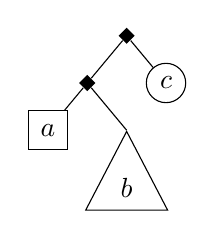
\begin{tikzpicture}[itermtree]
	\node[ap] {} child {
		node[ap] {} child { node[pure] {$a$} } child[subtrm] { node[subtrm] {$b$} }
	} child { node[term] {$c$} };
\end{tikzpicture}
\caption{$(\spure a \sap b) \sap \sterm c$ as a tree.}
\label{fig:iterm-ex}
\end{minipage}\hfill
\begin{minipage}[t]{0.46\textwidth}\centering
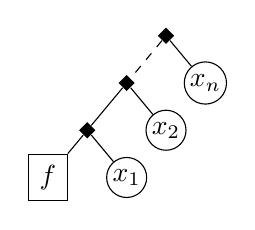
\begin{tikzpicture}[itermtree]
	\node[ap] {} child {
		node[ap] {} child {
			node[ap] {} child {
				node[pure] {$f$}
			} child { node[term] {$x_1$} }
		} child { node[term] {$x_2$} }
	    edge from parent [abbrv]
	} child { node[term] {$x_n$} };
\end{tikzpicture}
\caption{A term in normal form.}
\label{fig:iterm-nf-ex}
\end{minipage}
\end{figure}

Idiomatic terms are visualized naturally as trees.
This will be helpful in explaining term transformations.
Figure~\ref{fig:iterm-ex} shows the conventions:
Inner nodes correspond to $\sap$, leaves are either pure terms (boxes) or
opaque terms (circles).
Whole subterms may be abbreviated by a triangle.
A term has normal form if it consists of a single pure node to which a number
of opaque terms (or none) are applied in sequence.
Figure~\ref{fig:iterm-nf-ex} gives a general example.
A formal construction follows:

\begin{definition}[Normal form]
The set $\mathcal{N} \subset \mathcal{I}$ of idiomatic terms in normal form is
defined inductively as
\begin{gather}
	\spure x \in \mathcal{N}, \label{eq:nf-base}\\
	t \in \mathcal{N} \implies t \sap \sterm s \in \mathcal{N}. \label{eq:nf-step}
\end{gather}
\end{definition}

\begin{figure}\centering
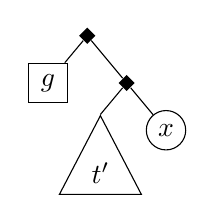
\begin{tikzpicture}[itermtree]
	\node[ap] {} child { node[pure] {$g$} } child {
		node[ap] {} child[subtrmn] { node[subtrm] {$t'$} } child { node[term] {$x$} }
	};
\end{tikzpicture}
\raisebox{10mm}{$\qquad\simeq\qquad$}
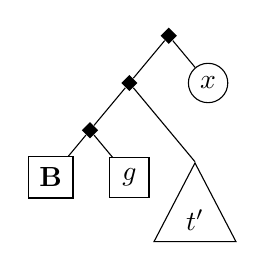
\begin{tikzpicture}[itermtree]
	\node[ap] {} child {
		node[ap] {} child {
			node[ap] {} child { node[pure] {$\mathbf{B}$} } child { node[pure] {$g$} }
		} child[subtrmf] { node[subtrm] {$t'$} }
	} child { node[term] {$x$} };
\end{tikzpicture}
\raisebox{10mm}{$\qquad\simeq\qquad$}
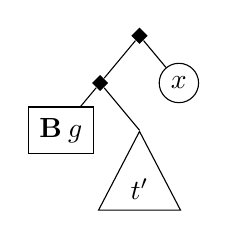
\begin{tikzpicture}[itermtree]
	\node[ap] {} child {
		node[ap] {} child { node[pure] {$\mathbf{B} \sapp g$} } child[subtrm] { node[subtrm] {$t'$} }
	} child { node[term] {$x$} };
\end{tikzpicture}
\caption{The ``pure-rotate'' step.}
\label{fig:pure-rotate}
\end{figure}

It is not entirely obvious how the normal form can be derived from equations
\eqref{eq:iterm-id}--\eqref{eq:iterm-xchng}.
Rewriting blindly with these is prone to infinite recursion.
Therefore we need a more controlled algorithm.
Consider an idiomatic term $t$.
If $t$ is a single pure term, then it is already in normal form.
The case $t = \sterm x$ is also easy:
Due to \eqref{eq:iterm-id}, we have $t \simeq \spure{(\sabs{x}{x})} \sap t$,
which is in normal form.
But in the case of $t = u \sap v$, various steps could be performed,
depending on the subterms.
We simplify the situation by normalizing each subterm recursively, so we get
an equivalent term $u' \sap v'$ where $u',v' \in \mathcal{N}$.

Now let us assume that $u'$ is just $\spure g$.
If $v'$ is also a pure term, they can be combined along \eqref{eq:iterm-morph}.
Otherwise, the term looks like the one on the left of Figure~\ref{fig:pure-rotate}.
As is shown there, the term tree can be rotated such that one opaque term moves
to the outer-most level.
This is the same equivalence as stated in \eqref{eq:pure-rotate}.
Because the remaining part again has the shape ``pure term applied to normal
form'', we proceed recursively.
In pattern-matching style, the transformation `pure-nf' reads
\begin{align}
	\operatorname{pure-nf}(\spure g \sap (f \sap x)) &=
		\operatorname{pure-nf}{(\spure{(\mathbf{B} g)} \sap f)} \sap x \\
	\operatorname{pure-nf}(\spure f \sap \spure x) &= \spure{(f x)}
\end{align}
\begin{lemma}\label{thm:pure-nf}
For all $g \in \mathcal{T}$ and $t \in \mathcal{N}$,
$\operatorname{pure-nf}(\spure g \sap t)$ is well-defined, and%
\/\footnote{$a \in S \simeq b$ abbreviates ``$a \in S$ and $a \simeq b$''.}
$\operatorname{pure-nf}(\spure g \sap t) \in \mathcal{N} \simeq \spure g \sap t$.
\end{lemma}
\begin{proof}
We prove all claims simultaneously by induction on $t \in \mathcal{N}$,
where $g$ is arbitrary.
\begin{prfcases}
\item Assume $t = \spure x$ for some $x \in \mathcal{T}$.
	Only the second equation applies, so we have
	\[ \operatorname{pure-nf}(\spure g \sap t) = \spure{(g \sapp x)}. \]
	All pure terms are in $\mathcal{N}$, and equivalence follows from
	\eqref{eq:iterm-morph}.
\item Assume $t = t' \sap \sterm x$ for some
	$t' \in \mathcal{N}$, $x \in \mathcal{T}$, and that the hypothesis holds
	for $t'$ and all $g$.
	Only the first equation applies, so
	\[ \operatorname{pure-nf}(\spure g \sap t) =
		\operatorname{pure-nf}(\spure{(\mathbf{B} g)} \sap t') \sap \sterm x. \]
	Instantiating the induction hypothesis, we find that
	\[ \operatorname{pure-nf}(\spure{(\mathbf{B} \sapp g)} \sap t') \in \mathcal{N} \simeq
		\spure{(\mathbf{B} \sapp g)} \sap t' \]
	is well-defined.
	$\mathcal{N}$ is closed under application to opaque terms \eqref{eq:nf-step},
	hence $\operatorname{pure-nf}(\spure g \sap t) \in \mathcal{N}$.
	Finally, we have
	\begin{align*}
		\operatorname{pure-nf}(\spure g \sap t) &\simeq
			\spure{(\mathbf{B} \sapp g)} \sap t' \sap \sterm x \\
		&\stackrel{\mathclap{\eqref{eq:pure-rotate}}}{\simeq}
			\spure g \sap (\spure t' \sap \sterm x) =
			\spure g \sap t. \qedhere
	\end{align*}
\end{prfcases}
\end{proof}

Going back to $u' \sap v'$, we assumed that $u'$ is a pure term.
The case where $v'$ is pure instead can be translated to the former by
\begin{equation}
	\operatorname{nf-pure}(f \sap \spure x) =
		\operatorname{pure-nf}{(\spure{((\sabs{x}\sabs{f}{f x}) \sapp x)} \sap f)} \\
\end{equation}
\begin{lemma}\label{thm:nf-pure}
For all $t \in \mathcal{N}$ and $x \in \mathcal{T}$,
$\operatorname{nf-pure}(t \sap \spure x)$ is well-defined, and
$\operatorname{nf-pure}(t \sap \spure x) \in \mathcal{N} \simeq t \sap \spure x$.
\end{lemma}
\begin{proof}
Follows from Lemma~\ref{thm:pure-nf} and \eqref{eq:iterm-xchng}.
\end{proof}

\begin{figure}\centering
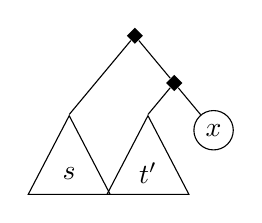
\begin{tikzpicture}[itermtree]
	\node[ap] {} child[subtrmf] { node[subtrm] {$s$} } child {
		node[ap] {} child[subtrmn] { node[subtrm] {$t'$} } child { node[term] {$x$} }
	};
\end{tikzpicture}
\raisebox{10mm}{$\qquad\simeq\qquad$}
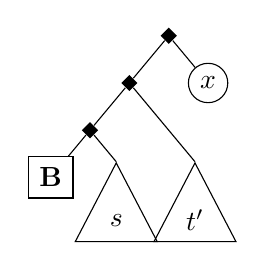
\begin{tikzpicture}[itermtree]
	\node[ap] {} child {
		node[ap] {} child {
			node[ap] {} child { node[pure] {$\mathbf{B}$} } child[subtrmn] {
				node[subtrm] {$s$}
			}
		} child[subtrmf] { node[subtrm] {$t'$} }
	} child { node[term] {$x$} };
\end{tikzpicture}
\caption{The ``rotate'' step.}
\label{fig:rotate}
\end{figure}

Finally, we look at general $u'$, $v'$.
A term rotation is useful again, see Figure~\ref{fig:rotate}.
Before recursion, we must normalize the subterm $\spure \mathbf{B} \sap s$.
But we already know how to do this: by `pure-nf'.
The base case is reached when $v'$ is a single pure term, which is the domain
of `nf-pure'.
The corresponding transformation is therefore
\begin{align}
	\operatorname{nf-nf}(g \sap (f \sap x)) &=
		\operatorname{nf-nf}{(\operatorname{pure-nf}{(\spure \mathbf{B} \sap g)} \sap f)} \sap x \\
	\operatorname{nf-nf}(t) &= \operatorname{nf-pure}(t) \quad\text{(otherwise)}
\end{align}
\begin{lemma}\label{thm:nf-nf}
For all $s,t \in \mathcal{N}$, 
$\operatorname{nf-nf}(s \sap t)$ is well-defined, and
$\operatorname{nf-nf}(s \sap t) \in \mathcal{N} \simeq s \sap t$.
\end{lemma}
\begin{proof}
The proof is similar to the one of Lemma~\ref{thm:pure-nf}, by induction on
$t \in \mathcal{N}$ and arbitrary $s \in \mathcal{N}$.
\begin{prfcases}
\item Assume $t = \spure x$ for some $x \in \mathcal{T}$.
	The second equation applies, so we have
	\[ \operatorname{nf-nf}(s \sap t) = \operatorname{nf-pure}(s \sap \spure x). \]
	Since $s \in \mathcal{N}$, the claim follows directly from Lemma~\ref{thm:nf-pure}.
\item Assume $t = t' \sap \sterm x$ for some
	$t' \in \mathcal{N}$, $x \in \mathcal{T}$, and that the hypothesis holds
	for $t'$ and all $s \in \mathcal{N}$.
	Only the first equation applies,
	\[ \operatorname{nf-nf}(s \sap t) =
		\operatorname{nf-nf} (\operatorname{pure-nf}(\spure \mathbf{B} \sap s) \sap t') \sap \sterm x. \]
	We have
	$\operatorname{pure-nf}(\spure \mathbf{B} \sap s) \in \mathcal{N} \simeq \spure \mathbf{B} \sap s$
	from Lemma~\ref{thm:pure-nf}.
	Thus we can instantiate the induction hypothesis, and the transformed term
	is indeed in normal form.
	Furthermore,
	\begin{align*}
		\operatorname{nf-nf}(s \sap t) &\stackrel{\mathclap{\text{(IH)}}}{\simeq}
			\operatorname{pure-nf}(\spure \mathbf{B} \sap s) \sap t' \sap \sterm x \\
		&\simeq \spure \mathbf{B} \sap s \sap t' \sap \sterm x \\
		&\stackrel{\mathclap{\eqref{eq:iterm-comp}}}{\simeq}
			s \sap (t' \sap \sterm x) = s \sap t. \qedhere
	\end{align*}
\end{prfcases}
\end{proof}

\begin{algorithm}[t]
\caption{Normalization of idiomatic terms.}
\label{alg:normalize}
\begin{gather*}
	\begin{align*}
		\operatorname{normalize}(\spure x) &= \spure x \\
		\operatorname{normalize}(\sterm x) &= \spure{(\sabs{x}{x})} \sap \sterm x \\
		\operatorname{normalize}(x \sap y) &=
			\operatorname{nf-nf}(\operatorname{normalize} x \sap \operatorname{normalize} y)
	\end{align*} \\[2ex]
	\begin{align*}
		\operatorname{nf-nf}(g \sap (f \sap x)) &=
			\operatorname{nf-nf}{(\operatorname{pure-nf}{(\spure \mathbf{B} \sap g)} \sap f)} \sap x \\
		\operatorname{nf-nf}(t) &= \operatorname{nf-pure}(t) \quad\text{(otherwise)}
	\end{align*} \\[2ex]
	\begin{align*}
		\operatorname{pure-nf}(\spure g \sap (f \sap x)) &=
			\operatorname{pure-nf}{(\spure{(\mathbf{B} g)} \sap f)} \sap x \\
		\operatorname{pure-nf}(\spure f \sap \spure x) &= \spure{(f x)}
	\end{align*} \\[2ex]
	\operatorname{nf-pure}(f \sap \spure x) =
		\operatorname{pure-nf}{(\spure{((\sabs{x}\sabs{f}{f x}) \sapp x)} \sap f)}
\end{gather*}
\end{algorithm}

Algorithm~\ref{alg:normalize} summarizes all pieces of the normal form
transformation.
`normalize' is the entry point and performs the main recursion mentioned in the
beginning.
We haven't proved the desired property for `normalize' yet, but this is just a
straightforward induction.

\begin{lemma}\label{thm:normalize}
For all $t \in \mathcal{I}$, $\operatorname{normalize} t$ is well-defined, and
$\operatorname{normalize} t \in \mathcal{N} \simeq t$.
\end{lemma}
\begin{proof}
By induction on $t$, Lemma~\ref{thm:nf-nf}, and equation \eqref{eq:iterm-id}.
\end{proof}

Until now, we only have considered the syntactic structure of idiomatic terms
together with the artificial relation $\simeq$, which is also based on syntax.
In order to define the semantics of idiomatic terms, we assume that we operate
in an equational theory $\Omega$ based on $\mathcal{T}$-terms, where
$=_\Omega\,\supseteq\,\termeq$ is an equivalence relation.

\begin{definition}[Idiomatic interpretation]\label{def:iterm-interp}
Let $\iota = \langle p, a \rangle$ with $p,a \in \mathcal{T}$.
The interpretation $\ldb t \rdb_\iota$ of the idiomatic term $t$ w.r.t. $\iota$
is defined as
\begin{align}
	\ldb \sterm t \rdb_\iota &= t, \\
	\ldb \spure t \rdb_\iota &= p \sapp t, \\
	\ldb s \sap t \rdb_\iota &= (a \sapp \ldb s \rdb_\iota) \sapp \ldb t \rdb_\iota.
\end{align}
$\iota$ is an idiomatic structure (in $\Omega$) iff
\begin{equation}
	\all{q r}{q \simeq r \implies \ldb q \rdb_\iota =_\Omega \ldb r \rdb_\iota}.
\end{equation}
\end{definition}

\begin{definition}\label{def:id-structure}
\begin{equation}
	\iota_\mathrm{id} = \langle \sabs{x}{x}, \sabs{f}{\sabs{x}{f \sapp x}} \rangle
\end{equation}
is the identity structure.
\end{definition}

% TODO lift \termeq to I

\begin{lemma}\label{thm:normal-form}
For all $t \in \mathcal{I}$, there is a unique term $t' \in \mathcal{N}$ such
that $t \simeq t'$.
\end{lemma}
\begin{proof}
Existence of the normal form is a corollary of Lemma~\ref{thm:normalize}.
In order to show that it is unique, we construct a relation
$R \subseteq \mathcal{I}\times\mathcal{I}$, such that
\begin{itemize}
\item for all idiomatic terms $s$ and $t$, $s \simeq t \implies (s,t) \in R$, and
\item for all terms in normal form $n$ and $n'$, $(n,n') \in R \implies n \termeq n'$.
\end{itemize}
$R$ is defined in two steps.
The first deals with the sequence of opaque terms,
\[
	\operatorname{opaq}(\spure x) = [], \quad
	\operatorname{opaq}(\sterm x) = [x], \quad
	\operatorname{opaq}(s \sap t) = \operatorname{opaq}(s) @ \operatorname{opaq}(t).
\]
Let $(s,t) \in R'$ if and only if $\operatorname{opaq}(s) = \operatorname{opaq}(t)$
pointwise.
Now assume $(s,t) \in R'$.
We can modify both terms such that all opaque terms are replaced by new pure
variables, say $\spure v_1,\dots,\spure v_n$.
The mapping is the same for both terms, i.e., the variable is determined by
the position in $\operatorname{opaq}(\_)$.
Let $s'$, $t'$ be these modified terms.
Then $(s,t) \in R$ if and only if
$\ldb s' \rdb_{\iota_\mathrm{id}} \termeq \ldb t' \rdb_{\iota_\mathrm{id}}$.

It remains to show that $R$ satisfies both properties.
\todo
\end{proof}

\begin{lemma}
\todo\ Every encoding of an applicative functor in $\Omega$ is an idiomatic
structure.
Especially $\iota_\mathrm{id}$ is an idiomatic structure.
\end{lemma}

\begin{definition}[Lifted terms]
$q \in \mathcal{I}$ is a lifting of $t \in \mathcal{T}$ if 
$\ldb q \rdb_{\iota_\mathrm{id}} =_\Omega t$.
\end{definition}

\begin{lemma}
Let $q$ be a lifting of $t$. The normal form $q'$ of $q$ can be written as
\[ q' = ( \cdots ((\spure t' \sap \sterm a_1) \sap \sterm a_2) \cdots ) \sap \sterm a_n. \]
Then $t' \sapp \vec a =_\Omega t$.
\end{lemma}
\todo

\section{Lifting with Combinators}\label{sec:combinators}

\subsection{Motivation}\label{subsec:combinator-motivation}

The normalization approach to solving lifted equations works only if the
opaque terms on both sides coincide.
This is not true for all equations of interest.
Let's revisit the set version of addition of natural numbers, $\oplus$ from
Example~\ref{exmp:set-intro}.
This operator is also commutative, so it should be possible to prove
\[ X \oplus Y = Y \oplus X. \]
After unfolding and normalization, we get
\begin{equation}\label{eq:comb-intro1}
	\pure{(\abs{xy}{x + y})} \ap X \ap Y = \pure{(\abs{yx}{y + x})} \ap Y \ap X.
\end{equation}
Clearly, this can't be solved with a standard congruence rule, because we would
have to to prove that $X$ is equal to $Y$.
Since we are concerned with transferring properties from a base domain,
we don't want to assume anything about those opaque subterms.

Hinze showed that such equations can be solved if certain \emph{combinators}
can be lifted.
Informally, combinators are functions which rearrange their arguments in a
specific manner.
We have already used two combinators, $\mathbf{I}$ and $\mathbf{B}$.
Lifting their defining equations (see Table~\ref{tab:combinators}) gives us
the identity and composition laws, respectively.
If the lifted combinator performs the same rearrangement with arbitrary
functorial values, one can translate that particular term structure between the
two layers.
In this case, we simply say that the combinator \emph{exists}.
To continue with~\eqref{eq:comb-intro1}, we could attempt to change the order of
$Y$ and $X$ on the right-hand side.
Note that these appear as arguments to a pure function.
The $\mathbf{C}$ combinator, also known as `flip' in functional programming,
does what we want: $\mathbf{C}fxy = fyx$.
The lifted equation is
\begin{equation}\label{eq:flip-lifted}
	\pure \mathbf{C} \ap f \ap x \ap y = f \ap y \ap x,
\end{equation}
and it is indeed true for set idiom!
From this we get
\begin{equation}\label{eq:comb-intro2}
	\pure{(+)} \ap X \ap Y = \pure{(\mathbf{C}(+))} \ap X \ap Y.
\end{equation}
The right-hand side is no longer the normal form of $Y \oplus X$, but still
a canonical form (which is why we distinguish these two).
But now the argument lists on both sides coincide.
We reduce to
\[ \abs{xy}{x + y} = \abs{xy}{y + x}, \]
which is extensionally equivalent to the base equation $x + y = y + x$.
The availability of equation~\eqref{eq:flip-lifted} is a quite powerful
condition, because it will allow us to permute opaque terms freely.
If permutations exist such that both sides of an equation in canonical form
align regarding their opaque terms, reduction by congruence is possible again.
This will again lead to the expected base equation.
However, the combinator $\mathbf{C}$ does not exist for all applicative functors.
For example, the order of values in a state monad may be significant.

\begin{table}\centering
\begin{tabular}{cll}
Symbol & Reduction \\
\hline
$\mathbf{B}$ & $\mathbf{B} x y z = x (y z)$ \\
$\mathbf{I}$ & $\mathbf{I} x = x$ \\
\hline
$\mathbf{C}$ & $\mathbf{C} x y z = x z y$ \\
$\mathbf{K}$ & $\mathbf{K} x y = x$ \\
$\mathbf{W}$ & $\mathbf{W} x y = x y y$ \\
$\mathbf{S}$ & $\mathbf{S} x y z = x z (y z)$ \\
$\mathbf{H}$ & $\mathbf{H} x y z = x y (z y)$ \\
\end{tabular}
\caption{Useful combinators.}
\label{tab:combinators}
\end{table}

Combinators appeared originally in the context of logic~\cite{curry68}.
They were studied because it is possible to write logical formulas without
variables using only applications of suitable combinators, as opposed to the
usual lambda calculus.
Table~\ref{tab:combinators} lists all combinators which are used throughout
this text, together with their defining equations.
There are certain sets of combinators which are sufficient to express all
lambda terms, $\{\mathbf{S,K}\}$ being one of them.
In other sets, only a limited part of terms is representable.
Hinze's Lifting Lemma shows that all terms and thus all equations can be
lifted while preserving the variable structure if $\mathbf{S}$ and $\mathbf{K}$
exist.
He also notes that other combinator set are useful, because there are idioms
where more than $\{\mathbf{B,I}\}$, but not all combinators exist.
Generally speaking, additional combinators enlarge the set of equations which
can be lifted.

The original proof of the Lifting~Lemma~\cite[11--14]{hinze10} uses induction
on the structure of idiomatic terms; it is not entirely obvious how it can
be generalized to other combinators sets, as it depends on the availability
of $\mathbf{K}$ to lift tuple projections.
In this section we present an implementation of this generalized lifting,
whose underlying concept works with arbitrary combinators.
However, it depends on an abstraction algorithm and the structure of
representable terms, which are difficult to derive automatically.
Therefore we will restrict ourselves to certain sets (``bases'') with
fixed algorithms, while understanding that the scope can be extended 
if needed.

\subsection{Generic Lifting}\label{subsec:generic-lifting}

We start with the relationship of combinators and lambda terms.
The equations in Table~\ref{tab:combinators} can be expressed as abstractions
$\mathbf{I} = \abs{x}{x}$ etc.
If we substitute occurrences of combinators in a term (signified by $=_\delta$),
new abstractions are introduced, which may be beta-reduced afterwards:
\[ \mathbf{WB} =_\delta (\abs{fx}{fxx})(\abs{gfx}{g(fx)}) =_\beta \abs{xy}{x(xy)}. \]
The question arises when and how this process can be reversed, meaning that
all abstractions are replaced by suitable combinators.
In Curry et.~al.~\cite[Section~6A]{curry68}, terms with variables, but no
abstractions are considered.
A syntactical operation is defined, denoted $[x]t$, where $t$ is such a term
and $x$ is a variable.
The desired property is that $x$ does not occur in $[x]t$, and
$([x]t)x =_{\delta\beta} t$.
Due to its notation, the operation is known as \emph{bracket abstraction}.
There is an obvious correspondence with lambda abstractions $\abs{x}{t}$.
Bracket abstraction however stands for a concrete applicative term, whereas
a lambda is an object of the syntax itself.
Replacing lambdas $\abs{x}{t}$ by brackets $[x]t$ performs the shift to a
combinator representation.
Curry et.\ al. give several possible definitions for bracket abstraction.
They note that these follow a scheme they refer to as an algorithm---a sequence
of rules, where each rule is a partial definition.
The rules may invoke abstraction recursively.
In particular, the following rules are used:

\begin{alignat}{2}
	\tag{$i$} [x]x &= \mathbf{I}, && \\
	\tag{$k$} [x]t &= \mathbf{K} t &&\qquad\text{if $x$ not free in $t$}, \\
	\tag{$\eta$} [x]tx &= t &&\qquad\text{if $x$ not free in $t$}, \\
	\tag{$b$} [x]st &= \mathbf{B}s([x]t) &&\qquad\text{if $x$ not free in $s$}, \\
	\tag{$c$} [x]st &= \mathbf{C}([x]s)t &&\qquad\text{if $x$ not free in $t$}, \\
	\tag{$s$} [x]st &= \mathbf{S}([x]s)([x]t). &&
\end{alignat}

The algorithm which consists of rules $(i)$, $(k)$ and $(s)$, in that order,
is written succinctly as $(iks)$.
The algorithm attempts to use the rules in their left-to-right order, applying
the first one whose restrictions are satisfied by the term at hand.
Each abstraction algorithm $A$ introduces a certain set of basic combinators,
which we refer to as $C(A)$.
It is sound only if certain postulates about those combinators, which are again
the equations in Table~\ref{tab:combinators}, are assumed.

\begin{example}\label{exmp:bracket-abs}
Using the $(iks)$ algorithm, one gets
\[ [x]xxy \stackrel{(s)}{=} \mathbf{S}([x]xx)([x]y)
	\stackrel{(s),(k)}{=} \mathbf{S}(\mathbf{S}([x]x)([x]x))(\mathbf{K}y)
	\stackrel{(i)}{=} \mathbf{S}(\mathbf{SII})(\mathbf{K}y). \]
Attempting to use the $(ik\eta bc)$ algorithm with the same abstraction
quickly comes to a stop:
\[ [x]xxy \stackrel{(c)}{=} \mathbf{C}([x]xx)y, \]
which is undefined.
\end{example}

As we can see, not all algorithms are total.
Therefore, there is a trade-off between the combinators required and the terms
for which abstraction is possible.
Bunder~\cite{bunder96} presents an analysis of the situation for certain
algorithms and combinator sets, based on rigorous definitions for term
translation and definability.
We will come back to this later, when we discuss how to order the variables in
an idiomatic term such that abstraction is defined.
For now, the concept of bracket abstraction with the example of rules
$(i)$--$(s)$ is sufficient.

Next, we attempt to transfer these concepts to idiomatic terms.
On the one hand, this is quite intuitive since the latter are also formed by
an application operator, and pure terms can be identified with constants.
But we do not have any ``idiomatic abstractions''.
Hinze actually defines these in terms of abstract combinators and an
extensionality property of the idiom.
For our purpose it is sufficient to work directly with bracket abstraction,
and we assume that all combinators are lifted, i.e. expressible as a pure term.
To clarify the following discussion, we adjust our $\mathcal{I}$ formalism
and replace opaque terms $\sterm x$ with variables.

\begin{definition}
The set of generic idiomatic terms $\mathcal{I}'$ is defined by
\begin{equation}
	\mathcal{I}' ::= \sivar \mathcal{V} \mid \spure \mathcal{T} \mid
		\mathcal{I}' \sap \mathcal{I}'.
\end{equation}
We reuse the congruence $\simeq$ from Definition~\ref{def:idiomatic-terms} for
generic terms.
The set of variables $\vars(t)$ of $t$ is defined as the set of all arguments
to $\sivar$ occuring in $t$.
The sequence of variables $\varseq(t)$ is defined similarly to $\operatorname{opaq}$.
Unlifting (see Definition~\ref{def:unlifting}) is also transferred, but uses
the variable $x$ in subterms $\sivar x$ instead of inventing new ones.
\end{definition}

Using this definition, it is clear what the rules for idiomatic abstraction
are:
\begin{alignat}{2}
	\tag{$i'$} [x]'(\sivar x) &= \spure \mathbf{I}, && \\
	\tag{$k'$} [x]'t &= \spure \mathbf{K} \sap t &&\qquad\text{if } x \not\in \vars(t), \\
	\tag{$\eta'$} [x]'(t \sap \sivar x) &= t &&\qquad\text{if } x \not\in\vars(t), \\
	\tag{$b'$} [x]'(s \sap t) &= \spure \mathbf{B} \sap s \sap [x]'t &&\qquad\text{if } x \not\in \vars(s), \\
	\tag{$c'$} [x]'(s \sap t) &= \spure \mathbf{C} \sap [x]'s \sap t &&\qquad\text{if } x \not\in \vars(t), \\
	\tag{$s'$} [x]'(s \sap t) &= \spure \mathbf{S} \sap [x]'s \sap [x]'t. &&
\end{alignat}
In general, the algorithm $A'$ on idiomatic terms is obtained from algorithm
$A$ on regular terms by lifting its rules in this fashion, preserving order.

Before we show the connection to the canonical form, there is one thing which
remains to be considered.
The interchange law allows us to move a variable out of the left subterm of
an application, given that the right subterm is pure.
This is not captured by rules $(b')$ and $(i')$, which are the only ones from
above which are valid in all idioms.
We define a combinator $\mathbf{T}xy = yx$ and the rules
\begin{alignat}{2}
	\tag{$t$} [x]st &= \mathbf{T}t([x]s) &&\qquad\text{if $t$ contains no variables}, \\
	\tag{$t'$} [x]'(s \sap t) &= \spure \mathbf{T} \sap t \sap [x]'s
		&&\qquad\text{if } \vars(t) = \emptyset.
\end{alignat}
Soundness of rule $(t')$ can be shown to be equivalent to the interchange law.
It is important to understand that $\mathbf{T}$ does not have to exist in the
idiom; these rules do not fit exactly in the pattern of the other rules.
The $\mathbf{T}$ combinator is also necessary to formulate the most generic
rule for the $\mathbf{W}$ combinator.
Without the interchange law, it could only be used for terms
$t \sap \sivar x \sap \sivar x$, i.e. those where the same variable is applied
twice in direct succession.
In an idiom, there may be arbitrary pure terms ``inbetween'' the variables.
We use the $(w)$ rule when the variable occurs in both operands of an application,
just like the $(s)$ rule.
\begin{alignat}{2}
	\tag{$w$} [x]st &= \mathbf{W}(\mathbf{B}(\mathbf{T}[x]t)(\mathbf{B}\mathbf{B}[x]s))
		&&\qquad\text{if $[x]t$ contains no variables}.
\end{alignat}
$(w')$ is derived similarly to the other rules.

As with ordinary terms, we demand a soundness property for idiomatic bracket
abstraction, namely that $[x]'t' \sap \sivar x \simeq_C t'$ holds true.
The definitions for the additional combinators $C$ get lifted to
$\spure \mathbf{I} \sap x \simeq_C x$ and so on, consistently extending our
congruence relation $\simeq$ to $\simeq_C$.
% FIXME \simeq is not consistent -- pure I <> pure x ~= pure x and pure I <> pure x = pure (Ix)

\begin{lemma}\label{thm:bracket-lifting}
Let $t' \in \mathcal{I'}$ be a generic idiomatic term, and $x \in \mathcal{V}$
a variable.
For an abstraction algorithm $A'$ consisting of a subset of rules $(i')$--$(t')$,
we have $\unlift{[x]'t'} = [x]\unlift{t'}$ and $[x]'t' \sap \sivar x \simeq_{C(A')} t'$,
assuming that $[x]'t'$ is defined.
Also, bracket abstraction does not add variables:
$\vars([x]'t') \subseteq \vars(t')$.
\end{lemma}
\begin{proof}
This statement uses that fact that the rules in $A'$ are very similar to those
of $A$.
In particular, rule $(r')$ is applied first when evaluating $[x]'t'$ iff rule
$(r)$ is applied first to $[x]\unlift{t'}$.
The remainder of the proof is a simple induction.
We show the case involving rule $(c')$ as an example, the other cases are similar.
Thus $t = s \sap u$ with $x \not\in \vars(u)$.
The induction hypothesis is
\[ \unlift{[x]'s} = [x]\unlift{s} \quad\text{and}\quad [x]'s \sap \sivar x \simeq_{C(A')} s
	\quad\text{and}\quad \vars([x]'s) \subseteq \vars(s). \]
Then we have
\[\begin{split}
	\unlift{[x]'t} \stackrel{(c')}{=} \unlift{(\spure \mathbf{C} \sap [x]'s \sap u)}
	= \mathbf{C} (\unlift{[x]'s}) (\unlift{u}) \\
	\stackrel{\text{(IH)}}{=} \mathbf{C} ([x]\unlift{s}) (\unlift{u})
	\stackrel{(c)}{=} [x](\unlift{s} \unlift{u})
	= [x]\unlift{t} \end{split}\]
and
\[\begin{split} [x]'t' \sap \sivar x = \spure \mathbf{C} \sap [x]'s \sap u \sap \sivar x
	\simeq_{C(A')} [x]'s \sap \sivar x \sap u \\
	\stackrel{\text{(IH)}}{\simeq}_{C(A')} s \sap u = t. \end{split}\]
\end{proof}

Now we can state the key obversation:
The successful abstraction of all variables in an idiomatic term leaves a
single pure term, per the homomorphism law.
Moreover, that term is equivalent to the result of applying the same abstraction
algorithm to the ``unlifted term''.
In principle, this works with arbitrary rules, as long as the statements of
Lemma~\ref{thm:bracket-lifting} hold true.

\begin{theorem}\label{thm:unlifting}
In the following, bracket abstraction uses algorithms $A$ and $A'$ with
a subset of the rules $(i)$--$(t)$ and $(i')$--$(t')$, respectively.
Let $t' \in \mathcal{I}'$ be a generic idiomatic term, and $x_1,\dots,x_n$
a permutation of the variables $\vars(t')$, or a superset thereof.
If $f = [x_1]\cdots[x_n]\unlift{t'}$ is defined for $A$, then
\begin{enumerate}
\item $[x_1]'\cdots[x_n]'t'$ consists only of applications of pure terms, and
\item the unique canonical form of $[x_1]'\cdots[x_n]'t'$ is $\spure f$;
\item $\spure f \sap \sivar x_1 \sap \cdots \sap \sivar x_n$ is a canonical
	form of $t'$;
\item replacing all combinators from $C(A)$ in $f$ with their definitions
	yields $f' =_{\beta\eta} \abs{x_1\cdots x_n}{\unlift{t'}}$.
\end{enumerate}
\end{theorem}
\begin{proof}
\begin{enumerate}
\item is due to $\unlift{([x_1]'\cdots[x_n]'t')} = f$ (induction and
	Lemma~\ref{thm:bracket-lifting}).
\item It is not difficult to see that a pure-only term $p$ has a unique canonical
	form, which is equal to $\spure \unlift{p}$.
\item We have $\spure f \sap \sivar x_1 \sap \cdots \sap \sivar x_n \simeq_{C(A)} t'$
	by induction, making repeated use of Lemma~\ref{thm:bracket-lifting}.
\item We show $[x_1]\cdots[x_n]\unlift{t'} =_{\delta\beta} \abs{x_1\cdots x_n}{\unlift{t'}}$.
	Note that $([x_i]p)x_i =_{\delta\beta} p$ for all terms $p$, and hence
	$[x_i]p =_\eta \abs{x_i}{([x_i]p)x_i} =_{\delta\beta} \abs{x_i}{p}$.
\end{enumerate}
\end{proof}

\begin{table}\centering
\begin{tabular}{lll} Base & Abstraction & Example idioms \\
\hline
$\mathbf{BI}$ & $(ibt)$ & state, list \\
$\mathbf{BIC}$ & $(ibtc)$ & set \\
$\mathbf{BIK}$ & $(kibt)$ & \\
$\mathbf{BIW}$ & $(ibtw)$ & either \\
$\mathbf{BCK}$ & $(kibtc)$ & \\
$\mathbf{BKW}$ & $(kibtw)$ & \\
$\mathbf{BICW}$ & $(ibtcs)$ & maybe \\
$\mathbf{BCKW}$ & $(kibtcs)$ & stream, $\alpha \to$ \\
\end{tabular}
\caption{Substructures of BCKW.}
\label{tab:combinator-bases}
\end{table}

Remember that we are interested in equations, which obviously consist of two
idiomatic terms.
We get to the base equation only if the same variable sequence is used for both
terms, and the assumptions of Theorem~\ref{thm:unlifting} are satisfied.
To complete the \emph{generic lifting} approach, we need a procedure for
determining the abstraction order.
Since this procedure has to depend on the abstraction algorithm, we fix the
combinator bases first.
Hinze focuses on $\mathbf{SK = BCKW}$ and $\mathbf{BICS = BICW}$, noting
that $\mathbf{BIC}$ is also relevant.
The set $\{\mathbf{B,I,C,K,W}\}$ and its subsets seem to be a good starting
point to cover relevant cases.
The additional combinators play an intuitive role:
$\mathbf{C}$ reorders variables, $\mathbf{W}$ duplicates them, and $\mathbf{K}$
permits abstraction over additional variables.
Table~\ref{tab:combinator-bases} lists all distinct subsets containing
$\mathbf{B}$ and $\mathbf{I}$, together with the abstraction algorithms we
propose.
We routinely ignore $\mathbf{T}$ when listing the combinators.
This highlights the connection with combinatorial logic, where some of those
bases have been studied.

The algorithms have been chosen in order to simplify the implementation, by
using the rules conditionally depending on the available combinators:
If $\mathbf{K}$ exists, start with $k$.
Then, for all bases, perform $ibt$.
If $\mathbf{C}$ (or $\mathbf{W}$) exists, add $c$ (or $w$), respectively.
However, if both do, use rule $s$ instead.
Below follows a detailed description of how the variable sequence can be found
in each base, and we justify the abstraction algorithms, meaning that the
preconditions of Theorem~\ref{thm:unlifting} are satisfied.
The function $\abseq_C(s,t)$ will denote the chosen sequence for terms $s$, $t$
in the context of base $C$.
% TODO talk about the examples in the table

\subsubsection*{$\mathbf{BI}$}\label{subsec:base-bi}

This is the minimal base which is available for all idioms.
We already know from Section~\ref{subsec:idiomatic-calculus} that there is only
one canonical form with respect to $\simeq$.
Therefore, there is exactly one permissible sequence:
\[ \abseq_\mathbf{BI}(s,t) = \varseq(s) = \varseq(t). \]
Equations where the two sequences differ are rejected.
If any other sequence could be used, we would get a different canonical form
per Theorem~\ref{thm:unlifting}, thus contradicting the previous result on
normal forms.
Focusing on a single abstraction step $[x_i]t_i$, $x_i$ must occur once in
$t_i$, and it is the right-most variable.
If $t_i$ is an application, there are two cases:
$x_i$ occurs in the right subterm, and rule $(b)$ is used successfully.
Otherwise, there can be no variable in the right subterm, so $(t)$ applies.
This confirms that algorithm $(ibt)$ is indeed acceptable for this base.

\subsubsection*{$\mathbf{BIC}$}\label{subsec:base-bic}

Bunder shows~\cite{bunder96} that $\mathbf{BIC}$-definable lambda terms are
those where each bound variable occurs excatly once, irrespective of their order.
His definition of a $C$-definable term $t$ (with combinator base $C$)
implies that there exists an abstraction algorithm such that $[x]s$ is defined
if $t = \abs{x}{s}$.
In particular, $(i\eta bc)$ is a valid algorithm.
From this it follows that we can choose the order in which we abstract, as long
as the corresponding variable occurs exactly one.
Note that our special $\mathbf{T}$ combinator is not considered there.
But as it can be simulated by the more powerful $\mathbf{CI}$, adding it to the
combinator base does not change anything.

In this base, we can work with all equations where the variable sequence of
one term can be reordered to the sequence of the second.
The order used for the abstraction is irrelevant, but it will be reflected
in the quantifier order of the base equation.
A simple choice is $\abseq_\mathbf{BIC}(s,t) = \varseq(s)$.
However note that we do not use the $(\eta)$ rule, but add the $(t)$ rule.
$(\eta)$ could be a considered as an optimization, since
$\abs{x}{yx} =_\beta \mathbf{B}y\mathbf{I}$, so $(b)$ and $(i)$ suffice.
Conversely, $(t)$ is a special case of $(c)$ with $(i)$, and adding it to the
algorithm next to $(c)$ just results in a slightly different combinator
representation.
We use this particular algorithm in order to simplify the implementation,
such that as much code as possible can be shared between the bases. 

\subsubsection*{$\mathbf{BCK}$ and $\mathbf{BICW}$}\label{subsec:base-bck-bicw}

These cases were also analyzed by Bunder.
For $\mathbf{BCK}$, the definable terms are those where each bound variable occurs
at most once, again ignoring the order.
In terms of bracket abstraction, $[x]y$ is then also defined if $x$ is not free
in $y$.
This allows us to extend the sequence with other variables.
We make use of this to deal with variables which only occur on one side of
an equation---it does not hurt to abstract over those too.
Hence, $\abseq_\mathbf{BCK}(s,t)$ can be any arrangement of the
set $\vars(s) \cup \vars(t)$.
The implementation uses a total order on the set of variables.
On the contrary, the definable terms of $\mathbf{BICW}$ have at least one
occurence of each bound variable; $[x]y$ can therefore be used if $x$ occurs
multiple times in $y$, and $x$ will not be free in $[x]y$.
Comparing this with $\mathbf{BIC}$, we loosen the restriction that variables
must not be repeated.
$\abseq_\mathbf{BICW}(s,t)$ must be an arrangement of $\vars(s) = \vars(t)$.
We can compute this by sorting the sequences again, and then trimming duplicates
which now are next to each other.

Bunder proposes the $(i\eta kbc)$ algorithm for $\mathbf{BCK}$, and
$(i\eta bcs)$ for $\mathbf{BICW}$; our rules are $(kibtc)$ and $(ibtcs)$,
respectively.
The comments on $(\eta)$ and $(t)$ from above apply here as well.
The only other difference is the position of $(k)$ in the list.
But $(k)$ on one side and $(i)$ and $(\eta)$ on the sider work with disjoint
sets of terms, so this is not an issue.

\subsubsection*{$\mathbf{BCKW}$}\label{subsec:base-bckw}

This base, which is logically equivalent to $\mathbf{SK}$, has some useful
properties:
$[x]y$ can always be defined, making it possible to use any abstraction
sequence, and in turn handle all equations.
In conjunction with Theorem~\ref{thm:unlifting}, we want to abstract all
free variables, though.
Therefore we determine the sequence as with $\mathbf{BCK}$, but the
term restriction is rescinded.
As for the abstraction algorithm, we use a variation of $(ik\eta bcs)$
from~\cite{curry68}.

\subsubsection*{$\mathbf{BIK}$, $\mathbf{BIW}$ and $\mathbf{BKW}$}\label{subsec:base-odd}

These bases do not appear to be significantly covered in the literature.
Since there is at least one useful example of an idiom with $\mathbf{BIW}$
combinators, we still shall implement and discuss them.
By adding the $\mathbf{K}$ combinator to $\mathbf{BI}$, additional variables
may be abstracted, but the other restrictions (order, single occurrence) remain.
Accordingly, we demand that $\abseq_\mathbf{BIK}(s,t)$ has $\varseq(s)$ and
$\varseq(t)$ as subsequences.
% TODO define "subsequence" somewhere?
For definiteness, we can limit it to the shortest sequence where variables
only in $s$ appear before those only in $t$, whenever there is an ambiguity:
$\abseq_\mathbf{BIK}(s,t) = \abseq'_\mathbf{BIK}(\varseq(s), \varseq(t))$,
\[ \abseq'_\mathbf{BIK}(a,b) = \begin{cases}
		x \cdot \abseq'_\mathbf{BIK}(a',b') &\text{if } a = x \cdot a', \; b = x \cdot b'; \\
		x \cdot \abseq'_\mathbf{BIK}(a',b) &\text{if } a = x \cdot a', \\
		x \cdot \abseq'_\mathbf{BIK}(a,b') &\text{if } b = x \cdot b', \\
		\langle \rangle &\text{if } a = b = \langle \rangle. \end{cases} \]
Trying rule $(k)$ in the beginning of the abstraction algorithm obviously takes
care of unused variables.

For the other bases, we simply take the abstraction algorithms as granted.
Based on that we analyze the set of defined bracket abstractions.
Since $\mathbf{W}$ duplicates variables, one might conjecture that a single
variable may now occur repeatedly.
No other variable may be interspersed in the lexical order, though, because
none of the available combinators reorder their arguments.
The following lemma proves that this intuition is correct.
In order to express it on the level of lambda terms, we overload $\varseq(x)$
in the obvious way.
We use the notation $x^n$ with sequence $x$ to stand for $n$ concatenated
copies of $x$.

\begin{lemma}
Let $x \in \mathcal{V}$ and $t \in \mathcal{T}$.
With algorithm $(ibtw)$, $[x]t$ is defined iff there is a natural number
$n \geq 1$ and a variable sequence $v$ such that
$\varseq(t) = v \mathbin{@} \langle x \rangle^n$, where $x$ does not appear in $v$.
The same statement holds true for algorithm $(kibtw)$, except that $n$ may be
zero as well.
\end{lemma}
\begin{proof}
The first part of the proof is concerned with the direction where $[x]t$ is
assumed to be defined.
We perform induction over the steps of the abstraction algorithm.
In the evaluation of $[x]s$ for a subterm $s$ of $t$, there are the following
cases:
If $(k)$ is used, then $x$ must not be free in $s$, thus $n = 0$ and $v = \varseq(s)$.
For $(i)$, we have $n = 1$ and $v = \langle\rangle$.
For $(b)$, there must be terms $u$ and $w$ with $s = uw$, and $x$ is not free
in $u$.
From the induction hypothesis we get adequate $n'$ and $v'$ for $[x]w$.
Then $n'$ and $\varseq(u) \mathbin{@} v'$ satisfy the conditions for $[x]s$.
Rules $(t)$ and $(w)$ are analogous:
For $(t)$, the side condition implies that $\varseq(w) = \langle\rangle$;
for $(w)$ we have $\varseq(w) = \langle x \rangle^k$ for some $k \geq 1$,
thus $\varseq(u) \mathbin{@} \varseq(w) = v' \mathbin{@} \langle x \rangle^{n'+k}$,
where $n'$ and $v'$ are from $[x]u$.

Now we show the other direction.
Assume that suitable $n$ and $v$ exist.
If $n = 0$, rule $(k)$ is used, because $x$ cannot be free in $t$.
Otherwise we assume $n \geq 1$ during an induction on the structure of $t$.
If $t$ is a variable, it must be $x$, so rule $(i)$ applies.
If it is an application $s = uw$ instead, there are three cases:
$x \not\in \vars(u)$, hence $v = \varseq(u) \mathbin{@} v'$ for some $v'$,
and $[x]w$ is defined by the induction hypothesis so we can use rule $(b)$.
If $\vars(w) = \emptyset$, $[x]u$ is defined and rule $(t)$ applies.
Otherwise, $\varseq(w) = \langle x \rangle^k$ with $k \leq n$ must hold,
so $(w)$ can be used.
\end{proof}

It follows that the abstraction sequences for $\mathbf{BIW}$ and $\mathbf{BKW}$
should be chosen like those of $\mathbf{BI}$ and $\mathbf{BIK}$, respectively;
but for each variable, a single span of repetitions in $\varseq(s)$ and
$\varseq(t)$ is allowed and treated like a single instance.

\subsection{Implementation}\label{subsec:combinator-implementation}

\todo

\section{Usage Examples}\label{sec:examples}

\subsection{User Interface}\label{subsec:detail-example}

\begin{figure}
\textbf{lemma} set\_plus\_assoc: $(X \oplus Y) \oplus Z = X \oplus (Y \oplus Z)$ \\
\textbf{proof} \\
\iindent \textbf{show} $X \oplus Y \oplus Z \subseteq X \oplus (Y \oplus Z)$ \textbf{proof} \\
\iindent\iindent \textbf{fix} $a$ \textbf{assume} $a \in X \oplus Y \oplus Z$ \\
\iindent\iindent \textbf{then obtain} $x$ $y$ $z$ \\
\iindent\iindent\iindent \textbf{where} elems: $x \in X$\hspace{1ex}$y \in Y$\hspace{1ex}$z \in Z$ \\
\iindent\iindent\iindent \textbf{and} sum: $a = x + y + z$ \\
\iindent\iindent\iindent \textbf{unfolding} set\_plus\_def ap\_set\_def \textbf{by} blast \\
\iindent\iindent \textbf{from} sum \textbf{have} $a = x + (y + z)$ \textbf{using} add.assoc \textbf{by} simp \\
\iindent\iindent \textbf{with} elems \textbf{show} $a \in X \oplus (Y \oplus Z)$ \\
\iindent\iindent\iindent \textbf{unfolding} set\_plus\_def ap\_set\_def \textbf{by} blast \\
\iindent \textbf{qed} \\
\textbf{next} \\
\iindent \textbf{show} $X \oplus (Y \oplus Z) \subseteq X \oplus Y \oplus Z$ \textbf{proof} \\
\iindent\iindent \emph{symmetric proof omitted \dots} \\
\iindent \textbf{qed} \\
\textbf{qed}

\caption{A semi-manual proof of the associative property of addition, lifted to sets.}
\label{fig:set-assoc-manual}
\end{figure}

This section demonstrates the user interface of our package by revisiting
Example~\ref{exmp:set-intro}.
We assume that $\oplus$ and $\ap$ for sets have been defined according to
equations \eqref{eq:set-plus} and~\eqref{eq:set-ap}, and ``set\_plus\_def'' and
``ap\_set\_def'' refer to these equations.
It is possible to prove the associative property with the standard facilities
of Isabelle/HOL, of course.
Figure~\ref{fig:set-assoc-manual} shows a canonical Isar proof.
Its structure follows natural reasoning about sets:
We prove set equality by showing mutual inclusion in both directions, each of
which is proven by the corresponding implication.
The operators in the term $a \in X \oplus Y \oplus Z$ are unfolded to obtain
nested set comprehensions.
The fully automatic proof method \emph{blast} is fortunately able to deduce
the relation to elements of the individual sets $X$, $Y$, $Z$.
Also note how the fact ``add.assoc'' is used in the middle---it states the base
equation.

The proof scheme can be adjusted for other properties.
It is, however, suitable only for the set idiom.
Inductive datatypes would likely need induction (or case splits for
non-recursive types), coinductive datatypes use coinduction, and so on.

Now we want to automate the full proof with our package.
First, it needs to be informed about the set idiom.
We provide a command to declare applicative functors:
\begin{isabelle}
	\textbf{applicative} set (C)
	\textbf{for} \\
	\iindent pure: $\abs{x}{\{x\}}$ \\
	\iindent ap: $\ap_\mathit{set}$ \\
	\textbf{unfolding} ap\_set\_def \textbf{by} fast+
\end{isabelle}
Its general syntax is
\begin{isabelle}
	\textbf{applicative} \textit{name} (\textit{combinator}, \dots) \\
	\textbf{for} \\
	\iindent pure: $\pure_f$\\
	\iindent ap: $\ap_f$ \\
	\textit{proof}
\end{isabelle}
The idiom will be made available under the \textit{name}.
It can be used to refer to the idiom manually in proofs.
The name is followed by an optional list of a subset of the symbols C, K, and W.
These declare which combinators are lifted, as explained in
Section~\ref{sec:combinators}.
The set idiom only lifts the $\mathbf{C}$ combinator.
The functions $\pure$ and $\ap$ imply the type scheme, see also
Section~\ref{subsec:proof-strategy}.
Finally, the idiom laws need to be proven.
The system presents the user with corresponding goals, which are solved by the
proof.
For sets, the goals are
\begin{align*}
1.\; & \All{x}{ \{\abs{x}{x}\} \ap x = x } \\
2.\; & \All{g f x}{ \{\abs{g f x}{g (f x)}\} \ap g \ap f \ap x = g \ap (f \ap x) } \\
3.\; & \All{f x}{ \{f\} \ap \{x\} = \{f x\} } \\
4.\; & \All{f x}{ f \ap \{x\} = \{\abs{f}{f x}\} \ap f } \\
5.\; & \All{f x y}{ \{\abs{f x y}{f y x}\} \ap f \ap x \ap y = f \ap y \ap x }
\end{align*}
In this example, the proof obligations are easily discharged by unfolding and
the automatic \emph{fast} prover.
After the command has been issued, the functor can be used in subsequent
commands.
Its data is stored in the theory context and thus can be imported along other
theory content.
This allows the construction of a reusable idiom library.

Next, the definition of $\oplus$ needs to be registered.
Otherwise, the proof method is not able to interpret a term like $X \oplus Y$ as
a composite idiomatic expression.
Lifted constants can be registered with the attribute \emph{applicative\_unfold},
which can be applied to facts $\mathit{lhs} = \mathit{rhs}$, where $\mathit{rhs}$
is an idiomatic expression.
The equation must be suitable for rewriting.

Finally, we are able to compress the proof to a single invocation of the new
proof method \emph{applicative\_lifting}.
The base equation is provided as a fact and is used automatically by the
supporting Isar framework:
\begin{isabelle}
\textbf{lemma} set\_plus\_assoc: $(X \oplus Y) \oplus Z = X \oplus (Y \oplus Z)$ \\
\textbf{using} add.assoc \textbf{by} applicative\_lifting
\end{isabelle}
The proof method can also be used when the variables in the lifted equation
have been instantiated with other terms.

\chapter{Conclusion}\label{sec:conclusion}

\section{Related Work}\label{subsec:related-work}

There already exist libraries for Isabelle/HOL which perform certain kinds of
lifting.
In this section, we want to highlight two of them and discuss how they compare
to our solution.
The first package~\cite{huffman05} implements a ``transfer principle''
specifically designed for nonstandard analysis (NSA).
It focuses on a fixed target type constructor, $\alpha\>\mathit{star}$.
Certain instances of $\alpha\>\mathit{star}$ constitute the nonstandard number
types.
For instance, the hypernatural numbers are elements of $\mathit{nat}\>\mathit{star}$.
Arithmetic operators and their properties have to be lifted in order to develop
their theory, which is automated by the transfer tactic.
Its goal is indeed very similar to ours, but just focused on one application.
Interestingly, the author of the NSA transfer package made use of the applicative
structure of $\alpha\>\mathit{star}$ to define lifted operators, as well as
predicates.
The latter is something the package presented in this report does not support.
We will briefly discuss it as a potential extension in the next section.

The automated lifting of properties is not generic over idioms, though.
This makes it possible to state all required rules directly as polymorphic
HOL theorems.
The tactic takes some lifted proposition, tries to find the base form by
deleting certain constants (compare this to our unfolding approach), and then
shows logical equivalence of the two by backchaining with suitable transfer
rules.
There is only little control by the ML implementation, as the process is mainly
guided by resolution with rule patterns.
Note that all parts of the input proposition go through the same process,
including logical operators such as quantifiers and equality.
This is a good place to mention that $\alpha\>\mathit{star}$ is based
on the function type $\mathit{nat} \funT \alpha$.
Therefore, all combinators can be lifted; variables can be handled by
resolution, because their order or duplication do not matter; all logical
operators are preserved by lifting (the lifted type can be thought of
as a collection of parameterized copies of the base formula).

We observe that the NSA transfer package is a lot more general than ours with
respect to lifted propositions, but is restricted to one particular idiom.
Many of the additional logical operators can only be lifted because of its
special properties.

The other package collection we want to discuss provides quotient types.
A quotient type is created from an existing type, the representation, and an
equivalence relation on it; its elements are isomorphic to the equivalence
classes.
The \emph{Lifting} and \emph{Transfer} packages~\cite{huffman13} constitute a
modular infrastructure for transferring results from the representation level
to the new type.
\emph{Transfer} finds and proves equivalences or implications between
propositions according to an extensible set of transfer rules.
These describe how two different functions (or type instances of the same
function) are related, given relations of their arguments.
Transfer is heavily driven by the type structure, following the principle of
relational parametricity.
The goal of \emph{Lifting} is to automate the specification of constants lifted
to quotient types.
Because this kind of lifting preserves properties by construction, these should
be carried over as well.
Therefore, the package uses transfer to relate the new constant with its
representation.

The relations used by transfer cannot express lifting to applicative functors.
Values of the latter are usually more complex than those of the base type,
instead of more abstract.
We would need to find relations which are strong enough to lift arbitrary
predicates.
This is clearly not possible for functors with effects.
To summarize, the actual lifting step of our package is very simple, because it
just considers pairs of extensionally equal functions;
the whole automation is necessary to extract these functions from idiomatic
expressions in the first place.
Transfer, on the other hand, preserves the term structure, but relates each
component of the term, and composes these relations according to the
transfer rules.


\section{Summary and Future Extensions}\label{subsec:summary-future}

We have successfully implemented Hinze's applicative lifting as a proof method
for Isabelle/HOL.
It can be instantiated for arbitrary idioms, making it a (hopefully) reusable
tool.
Since it supports several combinator sets, we take advantage of the individual
properties of the idioms.
The proof methods has been used to produce direct proofs of various algebraic
laws for streams and infinite binary trees.

The choice of a shallow embedding led to a rather compact implementation,
next to the registration infrastructure, which is necessary either way.
The highly polymorphic situation demands constant care for type parameter
instantations, which is tedious.
On the other hand, this is a problem for a deep embedding as well.

The current implementation is restricted to equations.
As we have seen above, certain idioms can lift quite a lot more.
A practical example are cancellation laws of a lifted binary operator, which
have the structure $\_ = \_ \implies \_ = \_$ (see also
Section~\ref{subsec:lifted-algebra}).
We had to prove these manually for the stream and infinite tree theories.
Again, variables make our live difficult:
The lifted assumption does not necessarily imply the base assumption for
\emph{all} instances, and we cannot eliminate the implication to continue
with the conclusion only.
It is not obvious which additional conditions are necessary or sufficient to
lift such properties.
We have seen that the ``power'' of the various idioms differs with respect to
combinators.
Those which are homomorphic to the environment functor (streams, etc.) seem to
be the most versatile.
It might be interesting to survey possible categorizations and how they lead
to further proof automation.

\pagebreak
\printbibliography

\end{document}
